% ============================================================================
%  Seccion "Conectividad de las redes: neuronas y clases de salida
%  desconectadas" -- corresponde a la Seccion 6 de
%  comparison/analisis_comparacion.md, reescrita en LaTeX con redaccion
%  narrativa de tesis.
%
%  Este archivo se puede usar de dos maneras:
%   (a) Compilarlo tal cual (standalone) para previsualizar el resultado en
%       PDF. Al compilarse solo, la seccion aparecera numerada como "1", no
%       como "6"; eso es normal y se corrige solo al integrarlo al documento
%       completo de la tesis, donde recupera su numero de seccion segun el
%       lugar donde se inserte.
%   (b) Copiar unicamente el contenido entre las marcas "INICIO DEL
%       CONTENIDO" y "FIN DEL CONTENIDO" hacia el archivo principal de la
%       tesis (via \input o pegado directo), si ese documento ya carga un
%       preambulo con graphicx, booktabs y compania.
%
%  Requiere los paquetes cargados abajo (graphicx, booktabs, hyperref, etc.).
%  Las tres figuras se referencian con ruta relativa a este archivo (carpeta
%  connectivity/ dentro de comparison/, generada por
%  ../analyze_connectivity.py); si el archivo se traslada a otra ubicacion,
%  ajustar esa ruta o copiar la carpeta connectivity/ junto con el .tex.
%
%  Las menciones a "Seccion 5" y "Seccion 7" dentro del texto son referencias
%  en texto plano (no \ref) a las secciones vecinas de
%  comparison/analisis_comparacion.md, que por ahora solo existen en
%  Markdown; si se renumeran al ensamblar la tesis completa en LaTeX, revisar
%  esas menciones.
% ============================================================================

\documentclass[12pt,a4paper]{article}

\usepackage[utf8]{inputenc}
\usepackage[T1]{fontenc}
\usepackage[spanish,es-tabla]{babel}
\usepackage[margin=2.5cm]{geometry}
\usepackage{graphicx}
\usepackage{booktabs}
\usepackage{caption}
\usepackage{amsmath}
\usepackage[hidelinks]{hyperref}

\begin{document}

% ==================== INICIO DEL CONTENIDO (para \input) ====================

\section{Conectividad de las redes: neuronas y clases de salida desconectadas}
\label{sec:conectividad}

Esta sección es, al igual que la síntesis descriptiva de la Sección 5, de carácter
descriptivo y no corresponde a ninguno de los seis ángulos estadísticos pareados de la
metodología (\texttt{docs/metodologia\_comparacion.md}): no se compara MOEACKF contra
SNSGAII mediante un test de hipótesis, sino que se caracteriza una propiedad estructural
de las redes que ambos algoritmos efectivamente producen. El análisis cubre la totalidad
de los 248 frentes archivados (ocho combinaciones de dataset y algoritmo, con 31 corridas
cada una), es decir, 1790 soluciones no dominadas en total, y fue generado mediante el
script \texttt{analyze\_connectivity.py} a partir de las columnas de pesos sinápticos
($w_0, \ldots, w_{D-1}$) de cada archivo \texttt{*\_front.csv}. Los datos completos que
sustentan esta sección quedan disponibles en
\texttt{comparison/connectivity/connectivity\_summary.csv} (agregados por combinación) y
en \texttt{comparison/connectivity/all\_solutions.csv} (una fila por cada solución
individual), de modo que cualquier cifra citada a continuación puede verificarse
directamente.

\subsection{Motivación y definiciones}
\label{sec:conectividad-motivacion}

La codificación del problema \texttt{SparseSNN} fija de antemano la topología de la red
—todas las neuronas y todas las sinapsis existen siempre— y delega en cada algoritmo la
decisión de cuáles sinapsis permanecen activas, a través del peso $w \in [0,1]$ asociado a
cada una de ellas: un valor $w = 0$ equivale a ``sin conexión'', exactamente el mismo
criterio que ya emplea el objetivo de dispersión $f_1$ (fracción de pesos activos, o
complejidad) durante la propia optimización. A partir de ese criterio se definen dos
nociones estructurales, evaluadas sobre las matrices reconstruidas $W_1$ (entrada hacia
capa oculta) y $W_2$ (capa oculta hacia salida) de cada solución del frente.

Se considera que una neurona oculta está \emph{muerta} cuando no posee ninguna entrada
activa ni ninguna salida activa, de modo que no puede formar parte de ningún camino
completo entre la entrada y la salida de la red. Esta condición se distingue de dos casos
más marginales —las neuronas de tipo \emph{sink}, con entrada activa pero sin ninguna
salida, y las de tipo \emph{source}, con salida activa pero sin ninguna entrada—, ambas
igualmente no funcionales pero considerablemente menos frecuentes en el corpus analizado.
Se dice, por otra parte, que una \emph{clase de salida está desconectada} cuando la
neurona de salida correspondiente presenta grado de entrada nulo, esto es, ninguna neurona
oculta le envía una conexión activa. Bajo el esquema de decisión de tipo ganador-toma-todo
que emplean las dos neuronas de salida de \texttt{SparseSNN}, una clase en esa situación
recibe siempre la misma entrada neta —nula—, de modo que la red queda, por construcción,
incapacitada para predecirla de forma informada, sin importar la entrada que reciba. A
este criterio simple se suma una verificación más estricta, que excluye los caminos que
dependen únicamente del peso de sesgo hacia la capa oculta y exige que la salida sea
alcanzable desde al menos una variable de entrada real, puesto que una neurona oculta cuya
única entrada activa es el sesgo tampoco responde en absoluto a los datos de entrada.

\subsection{Resultados agregados}
\label{sec:conectividad-resultados}

La Tabla~\ref{tab:conectividad-resumen} resume, para cada una de las ocho combinaciones de
dataset y algoritmo, la fracción media de neuronas ocultas muertas por corrida y dos
variantes del indicador de clase de salida desconectada: la proporción agrupada sobre
todas las soluciones del corpus, y la proporción restringida a la solución de mejor
accuracy de cada corrida, que es la que en la práctica se desplegaría. Agregando las
cuatro fuentes de datos por algoritmo, sin que esto constituya un test estadístico
adicional, MOEACKF exhibe un 74.4\% de neuronas ocultas muertas en promedio, un 56.5\% de
soluciones con al menos una clase de salida desconectada, y un 35.5\% de sus soluciones de
mejor accuracy afectadas (44 de 124 corridas); SNSGAII, por su parte, exhibe 87.4\%,
37.5\% y 26.6\% (33 de 124 corridas) respectivamente en los mismos tres indicadores.

\begin{table}[htbp]
\centering
\footnotesize
\caption{Indicadores de conectividad agregados por combinación de dataset y algoritmo,
sobre el total de 1790 soluciones de los 248 frentes archivados.}
\label{tab:conectividad-resumen}
\begin{tabular}{llrrrrr}
\toprule
Dataset & Algoritmo & Corridas & Soluciones &
\shortstack{\% muertas\\(media por corrida)} &
\shortstack{\% con salida\\desconectada\\(agrupado)} &
\shortstack{\% con salida desc.\\(mejor accuracy)} \\
\midrule
ds1 Australian & MOEACKF & 31 & 178 & 95.3 & 59.6 & 0.0 \\
ds1 Australian & SNSGAII & 31 & 228 & 91.0 & 31.1 & 0.0 \\
ds2 Climate    & MOEACKF & 31 & 205 & 89.2 & 91.7 & 61.3 \\
ds2 Climate    & SNSGAII & 31 & 106 & 98.3 & 100.0 & 100.0 \\
ds3 German     & MOEACKF & 31 & 171 & 88.5 & 90.6 & 80.6 \\
ds3 German     & SNSGAII & 31 & 283 & 85.7 & 31.1 & 0.0 \\
ds4 Sonar      & MOEACKF & 31 & 349 & 54.2 & 17.5 & 0.0 \\
ds4 Sonar      & SNSGAII & 31 & 270 & 85.7 & 25.2 & 6.5 \\
\midrule
\textbf{Todas} & \textbf{Todas} & \textbf{248} & \textbf{1790} & \textbf{86.0} & \textbf{47.1} & \textbf{31.0} \\
\bottomrule
\end{tabular}
\end{table}

El fenómeno es universal en un sentido trivial, y bastante menos universal en el sentido
que efectivamente importa para la tesis. En la totalidad de las 248 corridas, al menos una
solución del frente presenta alguna clase desconectada, pero esta cifra es en gran medida
mecánica: dado que $f_1$ es un objetivo minimizado explícitamente, el punto de menor
complejidad de cada frente casi siempre se ubica en el extremo de máxima dispersión o muy
cerca de él, y de hecho el 100\% de los frentes conserva su solución más dispersa con al
menos una salida desconectada. El indicador que sí resulta relevante es el de la última
columna de la Tabla~\ref{tab:conectividad-resumen}: la solución de mejor accuracy de cada
corrida presenta una clase de salida desconectada en ninguna de las 31 corridas de ds1 y
de ds4-MOEACKF, pero en las 31 corridas de ds2$\times$SNSGAII y en 25 de las 31 corridas de
ds3$\times$MOEACKF. Es decir, en al menos dos de las ocho combinaciones el algoritmo no
solo genera redes rotas como subproducto de explorar la dispersión, sino que su mejor
solución por accuracy es, de manera sistemática, una red que jamás puede predecir una de
las dos clases.

Se observa, además, una asimetría por clase que se repite de manera consistente dentro de
cada dataset. En ds2 (Climate) es casi siempre la clase 0 la que queda sin conexión (entre
91.7\% y 100\% de las soluciones, frente a un 26.8\%--38.7\% para la clase 1), mientras que
en ds3 (German) el patrón se invierte y es la clase 1 la que resulta sistemáticamente
desconectada (90.1\% en MOEACKF y 31.1\% en SNSGAII, frente a 31.0\% y 15.2\%
respectivamente para la clase 0). Esto es consistente con que ambos datasets presentan
clases desbalanceadas, y con que ninguno de los operadores de dispersión descritos en la
Sección~\ref{sec:conectividad-mecanismos} distingue entre clases al apagar pesos: la clase
minoritaria de cada dataset queda, en consecuencia, estructuralmente más expuesta a perder
toda su conexión de entrada.

Por último, la versión estricta del chequeo de conectividad —la que excluye los caminos
que dependen únicamente del sesgo— arroja un 51.8\% agrupado, frente al 47.1\% de la
versión simple. La diferencia es pequeña: la gran mayoría de las neuronas ``vivas'' ya
reciben al menos una variable de entrada real y no solo el sesgo, ya que los casos donde
la única entrada activa es el sesgo representan menos del 1\% de las neuronas ocultas de
todo el corpus. El criterio simple, en consecuencia, no subestima la magnitud del
problema.

\subsection{Ejemplos ilustrativos}
\label{sec:conectividad-ejemplos}

Los tres ejemplos siguientes se seleccionaron mediante una regla explícita aplicada sobre
la totalidad del corpus, y no de forma manual: el extremo estructural del fenómeno, el
caso que afecta directamente a la solución que en la práctica se desplegaría, y un caso
interior del frente que muestra que el fenómeno no está confinado a sus extremos. Los tres
provienen de datasets con a lo más 40 variables de entrada (ds1 y ds2), de modo que el
diagrama completo de la red resulta legible; en las tres figuras, las líneas dibujadas
corresponden a la totalidad de las conexiones activas de esa solución en particular.

\paragraph{Ejemplo A: extremo estructural.}
Corresponde a ds1 (Australian) $\times$ MOEACKF, corrida 0, el punto de menor complejidad
de su propio frente, con $f_1 = 0$: ninguno de los 680 pesos de la red está activo. Su
accuracy es de 57.2\%, sus 40 neuronas ocultas están todas muertas, y ambas clases de
salida presentan grado de entrada nulo, como se aprecia en la
Figura~\ref{fig:conectividad-ejemplo-a}. Se trata del óptimo puro del objetivo de
dispersión: una red completamente vacía que el algoritmo retiene en el frente de Pareto
exactamente porque minimiza $f_1$ sin que exista ninguna restricción de conectividad que
lo impida.

\begin{figure}[htbp]
\centering
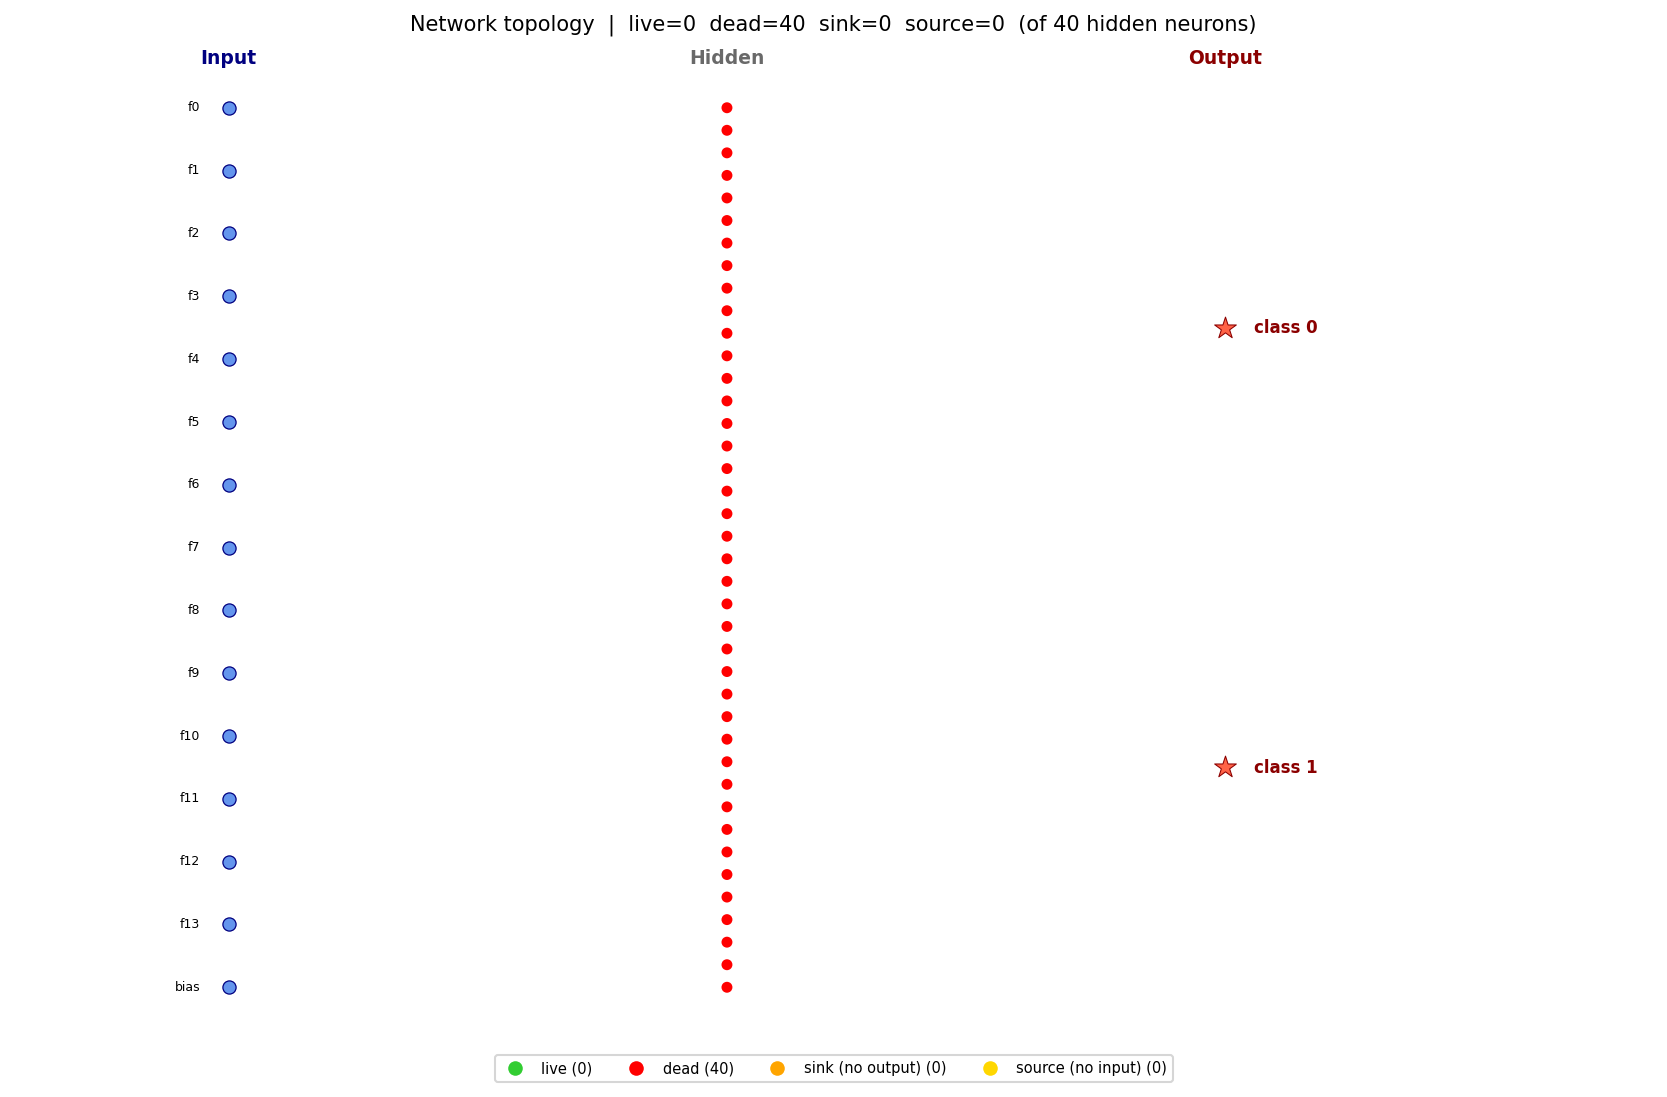
\includegraphics[width=0.85\textwidth]{connectivity/example_a_extreme.png}
\caption{Ejemplo A: red completamente vacía (ds1, MOEACKF, corrida 0). Las 40 neuronas
ocultas están muertas (en rojo) y ninguna de las dos clases de salida recibe conexión
alguna.}
\label{fig:conectividad-ejemplo-a}
\end{figure}

\paragraph{Ejemplo B: la solución que se desplegaría.}
Corresponde a ds2 (Climate) $\times$ SNSGAII, corrida 0, y a diferencia del Ejemplo A es la
solución de \emph{mejor accuracy} de su frente (92.1\%), con $f_1 \approx 0.0036$ —solo 3
de los 840 pesos de la red activos—. De las 40 neuronas ocultas, 39 están muertas; la
única viva alimenta exclusivamente a la clase 1, según se observa en la
Figura~\ref{fig:conectividad-ejemplo-b}. La clase 0 tiene grado de entrada nulo: bajo
decisión ganador-toma-todo, esta red —la más precisa de toda la corrida— nunca puede
predecir la clase 0, sin importar la entrada que reciba.

\begin{figure}[htbp]
\centering
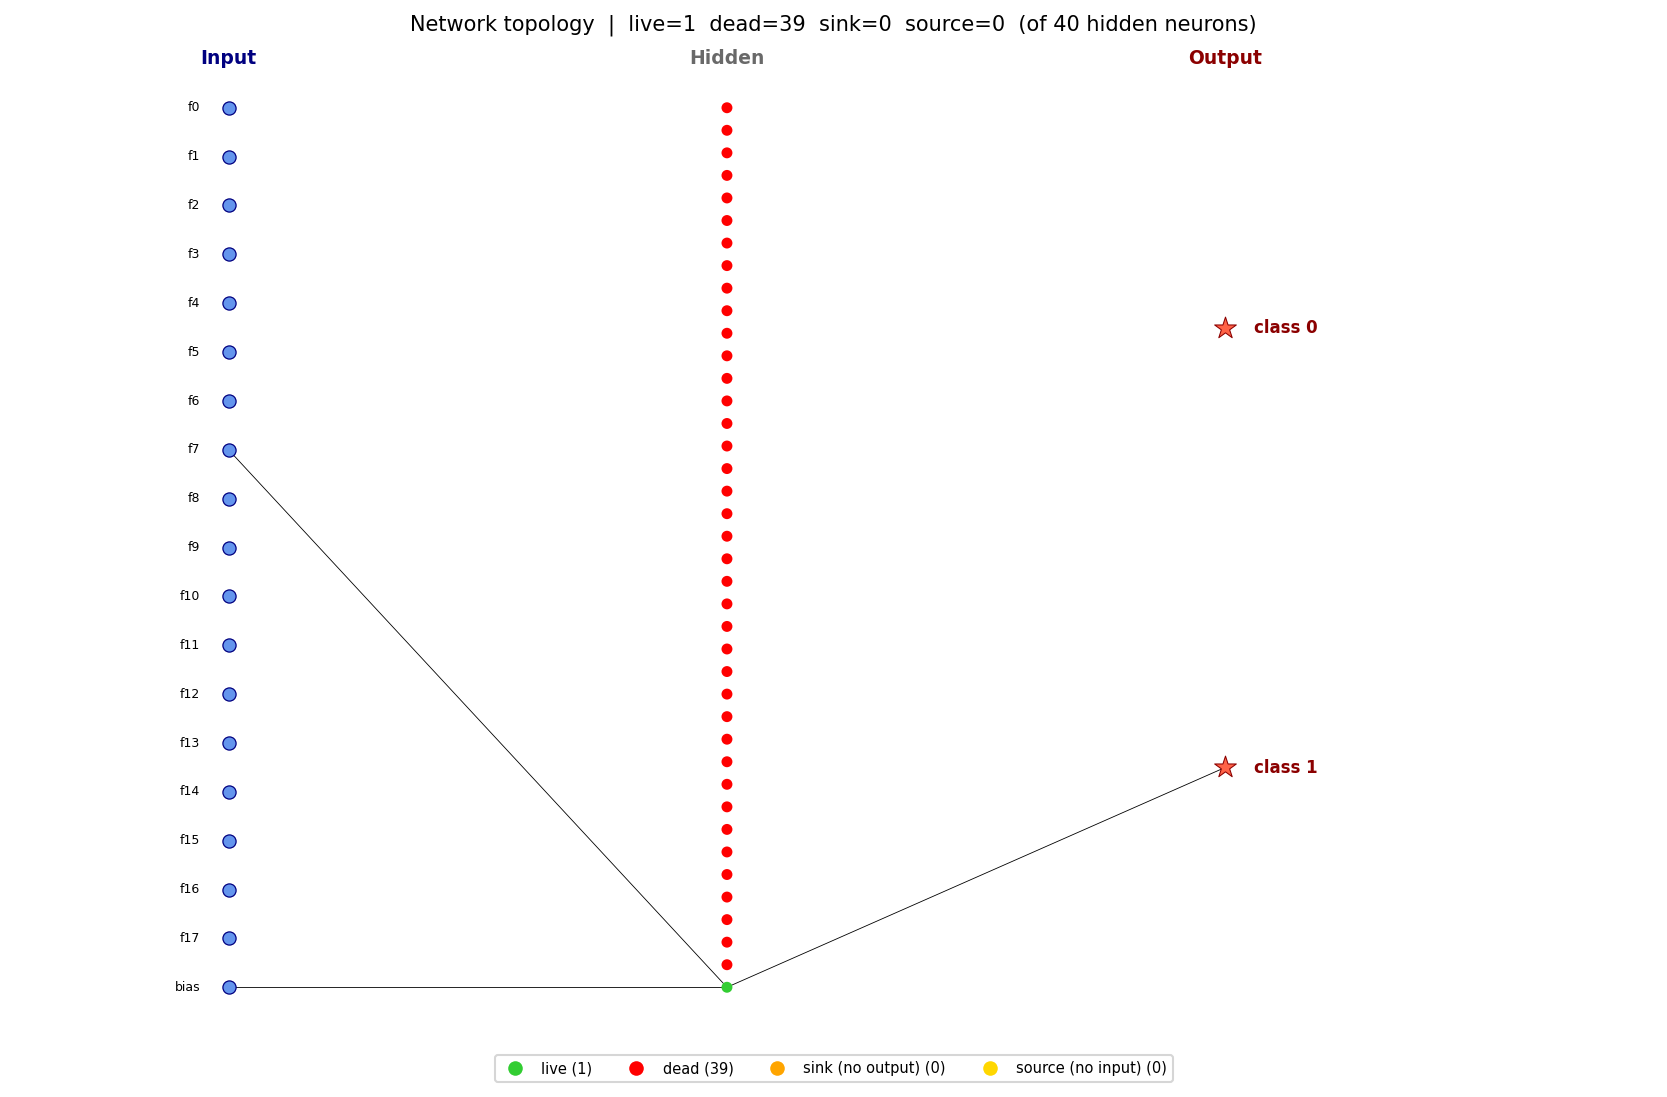
\includegraphics[width=0.85\textwidth]{connectivity/example_b_deployable.png}
\caption{Ejemplo B: única vía activa hacia la clase 1, en la solución de mejor accuracy de
su frente (ds2, SNSGAII, corrida 0). La clase 0 permanece sin ninguna conexión de
entrada.}
\label{fig:conectividad-ejemplo-b}
\end{figure}

\paragraph{Ejemplo C: caso interior del frente.}
Corresponde a ds1 (Australian) $\times$ MOEACKF, corrida 0, una solución interior de su
frente —ni la más dispersa ni la de mejor accuracy—, con accuracy de 69.6\% y solo 2 de
los 680 pesos activos. Como se aprecia en la Figura~\ref{fig:conectividad-ejemplo-c},
presenta el mismo patrón que el Ejemplo B a menor escala: una única neurona oculta viva
que alimenta solamente a la clase 1, mientras que la clase 0 vuelve a presentar grado de
entrada nulo. Este ejemplo muestra que el fenómeno no está confinado a los extremos del
frente de Pareto, sino que también aparece en sus soluciones intermedias.

\begin{figure}[htbp]
\centering
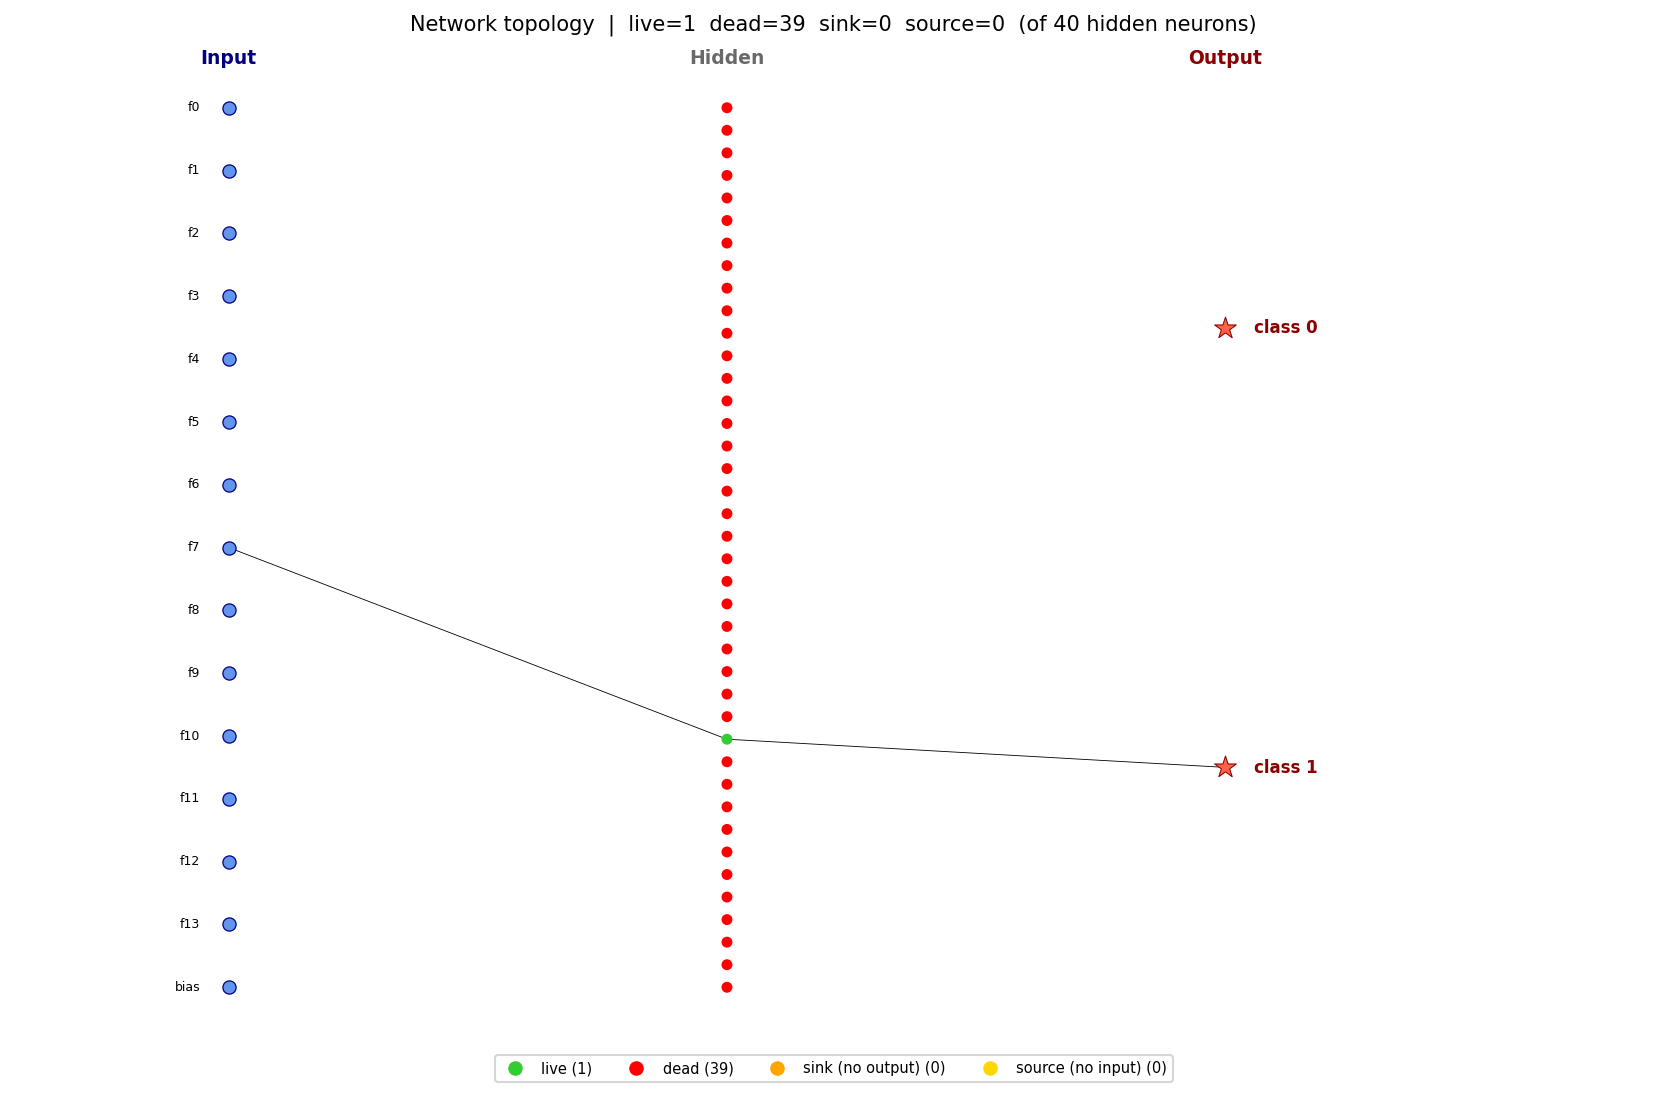
\includegraphics[width=0.85\textwidth]{connectivity/example_c_interior.png}
\caption{Ejemplo C: caso interior del frente con la clase 0 desconectada (ds1, MOEACKF,
corrida 0).}
\label{fig:conectividad-ejemplo-c}
\end{figure}

\subsection{Por qué es un producto del algoritmo, y no del azar}
\label{sec:conectividad-mecanismos}

Ninguno de los mecanismos que apagan pesos durante la optimización posee noción alguna de
a qué neurona o a qué salida pertenece cada sinapsis: todos operan gen por gen, o sobre un
conteo u objetivo global de dispersión, sin considerar en ningún momento la estructura del
grafo subyacente. En la inicialización de \texttt{SparseSNN}, cada gen se apaga de forma
independiente con una probabilidad aproximada del 50\%, un procedimiento puramente
bernoulliano que no distingue entre los pesos que alimentan una neurona oculta y los que
alimentan una neurona de salida. En el caso de SNSGAII, el operador de inicialización
\texttt{VSSPS} construye, en cambio, una máscara de densidad organizada en franjas
contiguas del vector de decisión, capaz de apagar de una sola vez filas completas de
$W_1$, es decir, neuronas ocultas enteras; su operador de mutación de dispersión, formado
por \texttt{SPM} y \texttt{sm2target}, muta el nivel de dispersión objetivo de todo el
individuo y luego apaga o reactiva pesos al azar hasta alcanzar ese nuevo nivel, otra vez
sin mirar a qué neurona pertenece cada uno; y su operador de cruce \texttt{SSBX}
intercambia al azar, entre los dos hijos, el estado activo o inactivo de los genes en los
que los padres difieren. MOEACKF, por su parte, construye la máscara binaria de su primera
generación mediante el procedimiento \texttt{PriorAnalysis}, que activa un número
aleatorio $k \in [1, D]$ de variables sobre el total de la red —pudiendo dejar tan solo una
sinapsis activa de las $D$ totales—, sin ninguna garantía de que ese reducido conjunto
toque siquiera una neurona de salida.

La huella que deja cada algoritmo en los resultados agregados de la
Sección~\ref{sec:conectividad-resultados} resulta consistente con su mecanismo
particular. La máscara binaria de MOEACKF, gobernada por un parámetro $k$ global e
indiferente al segmento del vector que activa, deja proporcionalmente más soluciones con
alguna clase de salida completa sin ninguna conexión (56.5\% frente al 37.5\% de SNSGAII);
la máscara en franjas contiguas de SNSGAII, en cambio, apaga con mayor frecuencia neuronas
ocultas completas (87.4\% muertas en promedio, frente al 74.4\% de MOEACKF). Que dos
mecanismos de dispersión distintos produzcan dos huellas de falla igualmente distintas es
un indicio adicional de que el patrón observado proviene del diseño particular de cada
operador, y no de una coincidencia compartida entre ambos algoritmos.

\subsection{Trabajo futuro recomendado}
\label{sec:conectividad-trabajo-futuro}

Ninguna de estas causas se corrige evaluando de mejor manera la red resultante, sino
interviniendo directamente en los operadores que deciden qué sinapsis permanecen activas.
Queda como trabajo futuro —no implementado ni evaluado en el marco de esta tesis— explorar
al menos cuatro direcciones de modificación sobre la codificación y los operadores
actuales de \texttt{SparseSNN}, MOEACKF y SNSGAII. La primera consiste en incorporar un
operador de reparación que se aplique después de cada mutación o cruce y antes de evaluar
al individuo, capaz de detectar neuronas muertas o salidas con grado de entrada nulo y
reactivar determinísticamente al menos una conexión hacia cada una de ellas. La segunda
apunta a una inicialización consciente de la conectividad, que garantice, al construir
cada individuo inicial, al menos un camino activo completo entre la entrada y cada clase
de salida, en lugar de apagar genes de forma uniforme o por franjas sin considerar la
estructura resultante. La tercera dirección consiste en operadores de mutación y cruce que
protejan explícitamente la última conexión activa hacia una neurona de salida, o hacia una
neurona oculta que constituya el único puente hacia esa salida, impidiendo que se apague
por azar. La cuarta, finalmente, propone incorporar la conectividad de entrada a salida
directamente en la función de aptitud —ya sea como objetivo adicional o como
penalización— o como restricción de factibilidad, en lugar de dejar que dicha conectividad
emerja únicamente como efecto colateral de minimizar $f_1$.

% ==================== FIN DEL CONTENIDO (para \input) ====================

\end{document}
